
\chapter{QUADRO TEÓRICO}

% Discussões => Leitura das teorias => Colocar em forma de resumos => Mostrar o
% PORQUE?

% Redes de Computadores e a Internet - 4a Edição - página 33
\par Segundo \citeonline{Redes_Comer}, Há um crescimento muito grande das redes
de computadores na atualidade, no início, há 20 anos, existia apenas um número
limitado de usuários na redes, hoje torna-se essencial o uso da rede de
computadores em todos os setores como, négocios, propaganda, transporte,
planejamento, faturamento, economia, pesquisas e produção. Atualmente as
instituições de ensino vem fazendo uso das redes, para facilitar o acesso a
informação, disponibilizando acervos digitais, consultas a acervos físicos,
boletins, onde alunos e professores possam interagir. A redes de computadores
também é usada em níveis federais, estaduais e militares, deixando assim a
clareza de que a rede de computadores está em todas as partes.

%------------------------------------------------------------------------
% Ligação da teoria com a pesquisa => porque o motivo da escolha

\par Ainda segundo o autor acima, este crescimento das rede tem influência no
setor econômico, devido ao meios disponíveis para comunicação, denomindo como \textit{telecommuting},
que modificou a meneira com que os negócios são feitos. Conforme a evolução das
redes de computadores, foi gerando a necessidade do mercado em haver serviços e
produtos relacionados, criando um mercado vasto, gerando novos empregos na área
tecnológica, levando em consideração que as empresas necessitam de colaboradores
que tenham conhecimentos em informática, que saibam planejar, comprar, instalar,
operar, gerenciar os sistemas de hardware e software e infraestrutura de redes e
inter-redes. 

%------------------------------------------------------------------------
\section{Rede de Computadores}

% história de Redes

%Comunicacao de Dados e Redes de Computadores-Behrouz A. Forouzan -       
%  página 46 no pdf;

\par Para \citeonline{Redes_Forouzan}, Ainda na décda de 60, os computadores de
grande porte conhecidos como \textit{mainframes}, tralhavam izolados, nas
empresas relacionadas a pesquisa, então a ARPA (\textit{Advanced Research
Projects Agency}), uma agência interna detro do departamento de defesa dos
Esdados Unidos, queria facilitar o compartilhamento de dados entra as
instituições de pesquisa, assim também diminuir os custos e esforços.
No encontro realizado em 1967 na ACM (\textit{Association Computing
Machinery}), foi apresentado a ideia de uma rede de comunicação de computadores
pela ARPA, o nome da pequena rede de computadores foi ARPANET, a principal idéia
da ARPANET era fazer com que pequenos computadores possam se comunciar entre si
, idependente de seus frabricantes, criando uma rede de comunição heterogênia,
para a comunicação ser estabelecida faz-se necessário o uso de uma inteface
denomida IMP (\textit{Interface Message Processor}), onde os computadores locias
acessavam a interface a a interface posibiliatava a comunição entre eles.

\par Ainda de acordo com o autor acima, a concretização da ARPANET só veio em
1969, quando foi criado pontos com o IMP, na UCLA (\textit{University of
California}) em Los Angeles, na \textit{University od Utah} ,na UCSB
(\textit{University of California}) em Santa Barbara e em SRI
(\textit{Stanford Research Institute}), para poder fazer controle
entre os computadores foi criado um software nomeado NCP (\textit{Network
Control Protocol}). Com a colaboração de dois participante do projeto ARPANET,
Vint Cerf e Bob Kahn, criaram o então conhecido \textit{Internetting Project}. 
Em 1973, em um artigo, que falava sobre o protocolo de controle de
transmissão (\textit{Transmission Control Protocol} - TCP),eles criaram esse
novos protocolos, o qual tem uma estrutura forte e que possui uma boa estrutura
de comunicação, de envio e recebimento de pacotes ponto a ponto em uma rede de
computadores, combriam também neste artigo conceitos de encapsulamento,
datagramas e funções \textit{gateway}. Logo o protocola TCP seria dividido pela
autoridades da área de informática, onde o IP (\textit{InternetWorking
Protocol}) e o TCP , seriam responsáveis por funções diferentes, o IP ficaria
incumbido pelo roteamento de datagrama, já o TCP ficaria com o alto escalão, na
segmentação, detecção de erros e reagrupamento. Após a divisão o TCP, tornando o \textit{InternetWorking
Protocl} conhecido com TCP/IP.

% Guia Administrador Redes Linux -  página 34

De acordo com \citeonline{Redes_Guia_adm_redes_linux}, O protocolo foi aceito como
padrão em 1983, assim o servidores passaram a utiliza o TCP/IP como protocolo
padrão, desta maneira a pequena ARPANET expandiu e tornou-se a Internet,
extinguindo propriamente dito a ARPANET em 1990.


%Redes de Computadores e a Internet - 5a Edição - página 27
%\par 

%Redes de Computadores curso completo - página 27

%\par 

%------------------------------------------------------------------------
% O que é o Protocolo
%Redes de Computadores e a Internet - 5a Edição - página 32
%\par 


%------------------------------------------------------------------------
% O que é o TCP

%\section{\textit{Transmission Control Protocol}}

%\par


%------------------------------------------------------------------------
% O que é o UDP

%\section{\textit{User Datagram Protocol}}

%\par


%------------------------------------------------------------------------
% O que é o IP

%\section{\textit{Internet Protocol}}

%\par

%------------------------------------------------------------------------
% história do SNMP


\section{\textit{Simple Network Management Protocol}  }

\par  O lançamento do SNMP foi feito em 1988, o objetivo do SNMP é fazer o
gerenciamento de redes, que constantemente está crescendo, baseados no padrão de
dispositivos IP, o SNMP ainda consciste em um grupo de operações de
gerenacimento que pode ser executado remotamente.

\par Para \citeonline[p.1]{SNMP_Schmidt_Mauro},

\begin{citacao}
	\par O núcleo do SNMP é um conjunto simples de operações (e das informações
	obtidas por essas operações) que permitem ao administrador modificar o estado
	de alguns dispositivos baseados em SNMP. Por exemplo, é possível utilizar o
	SNMP para encerrar uma interface em um roteador ou verificar a velocidade
	operacional de uma interface de Ethenet. O SNMP pode até monitorar a
	temperatura de um computador e avisar quando ela estiver muito alta.
\end{citacao}

\par Normalmente há uma associação com gerenciamento de roteadores com o SNMP,
mais podemos afimar que o SNMP pode fazer gerência de vários dispositivos em uma
rede de computadores não somente os roateadores, está associação deve se ao seu
antecessor o SGMP (\textit{Simple Gatway Management Protocol}), que fora criado
para apenas gerir roteadores de internet. O SNMP pode gerenciar vários
dispositivos como impressoras, fontes de energia, notebook, desktops,
roteadores e sistemas Windows, Linux e Unix. Desta maneira torna-se possível o
gerenciamento de qualquer dispositivo que esteja com o aplicativo SNMP em
execução e que possibilite a recuperação de informações do SNMP, a recuperação é
extendida não somente a hardware mais a softwares, servidores e bancos de dados.

\par O SNMP também é capaz de gerenciar todas a rede e não exclusivamente
dispositivos separadamente, tais como roteadores, hosts e impressoras, etc.
Através do RMON (\textit{Remote Network Monitoring}) para entender como a rede
funciona e como cada componente separadamente afeta a rede de computadores como
um todo, há a possibilidade de fazer com o que o RMON gerencie não somente a
rede LAN, mais também as interfaces WAN (\textit{Wide Area Network}).

% Inserir as Versões snmp essencial pg. 8


%------------------------------------------------------------------------
% história do MRTG

%\section{MRTG}

%\par



%------------------------------------------------------------------------
% história do Nágios

%\section{Nagios}

%\par



%------------------------------------------------------------------------
% história do JAVA

\section{Java}

\par  Na revolução dos computadores a que mai contribuiu para o desenvlvimento
foi a criação de microcomputadores pessoais, que possibilitou que milhões de
pessoas, modificandondo assim a vida das pessoas bem como a maneira com que os
negócios são geridos.

\par segundo \citeonline[p.6-7]{Java_Deitel_6edition},

\begin{citacao}
	Os microcomputadores têmum impacto profundo em dispositivos inteligentes
	eletrônicos voltados para o consumidor. Reconhecendo isso, a Sun Microsystems,
	em 1991, financiou u projeto de pesquisa corporativa interna com o codinome
	Green, que resultou no desenvolvimento deuma linguagem baseada em C++ que seu
	criador, James Gsoling, chamou de Oak em homenagem a uma árvore de carvalho
	vista por uma janela na Sum. Descobriu-se mais tarde que já havia uma linguagem
	de computador chamada de Oak. Quando uma equipe da Sum visitou uma cafeteria
	local, o nome Java (cidade de origem de um tipo de café importado) foi sugerido
	e o nome pegou.
\end{citacao}

\par O projeto Green, por não se desenvolver o mercado de dispositivos voltados
a população no início da década de 90. Mais com a explosão causada pela expansão
da web em 1993, a Sum investiu em novas funcionalidades, como conteúdo dinãmico,
animações e interatividade, colocando o java na web.

\par Graças a um conferência em 1995, hoje o java é utilizado em diversos
setores, como de telecomunição, aplicativos mobile, desktop e web, ainda
aplicativos que são utilizados em pager, tvs e monitores.


%------------------------------------------------------------------------
% história do ICONIX - introdução a metodologia

% Livro UML Metodologia e ferramentas case página 375

\section{ICONIX}

\par  Segundo \citeonline{UML_Silva_Videira}, O ICONIX fora desenvolvido pela
empresa ICONIX \textit{Software Engineering}, cujo o projeto tem como o foco é a
diponibilização e crição de materiais que possão ser utilizados em linguagem e
tecnologias de objetos, como por exemplo: COBRA, COM e JAVA.O ICONIX é um
processo que deixa mais prático  desenvolvimento de software, trata-se de uma metodologia de
desenvolvimento de software. Ele possui quatro tarrefas principais que que são:

\begin{itemize}
  \item Análise de requisitos
  \item Análise e desempenho preliminar
  \item Desenhos
  \item Implementação
\end{itemize}

\par A ordem ao qual foi mencionada é a qual
deve ser seguida. Segundo \citeonline[p.376]{UML_Silva_Videira},

\begin{citacao}
	A metodologia consiste na produção de um conjunto de artefactos que
    retratam as visões dinâmica e estática de um sistema, e que vão sendo
 	desenvolvidos incrementalmente e em paralelo, os modelos da estática
	e os modelos da dinâmica.
\end{citacao}



%                      Texto Original
%ICONIX Process is a scenario-based approach; the primary mechanism for
% decomposing and modeling the system is on a scenario-by-scenario basis. But when you use ICONIX Process,
%your goal is to produce an object-oriented design that you can code from.
% Therefore, you need to link the scenarios to objects. You do this by writing the use cases using the domain model
%that you created in the previous step.



\par Para \citeonline{UML_Case_Driven}, O ICONIX é um processo que faz um
tratamento baseado em cenário, este tratamento basea-se em um método de abordagem principal
que faz a decomposição e modelagem de um sistema com funcdamentação em
cenário-a-cenário. Ao faz uso do ICONIX cria-se a finalidade de implementação de
projetos orientados a objeto, assim podendo usar os diagramas com alicerce para
a programação. Para isso é necessário vincular todos os cenários a objetos,
pode-se criar este modelo ao escrever o caso de uso utilizando o modelo de
domínio.

%                      Texto Original
%Domain modeling is the task of building a project glossary, or a dictionary of
% terms used in your project (e.g., an Internet bookstore project would include domain objects such as Book,
%Customer, Order, and Order Item). Its purpose is to make sure everyone on the
% project understands the problem space in unambiguous terms. The domain model for a project defines the
%scope and forms the foundation on which to build your use cases. The domain
% model also provides a common vocabulary to enable clear communication among members of a project
%team. Expect early versions of your domain model to be wrong; as you explore
% each use case, you’ll “firm up” the domain model as you go.

\par A concepção de um glossário do projeto, denomina-se modelagem de domínio,
também pode ser descrito como dicionário de termos aplicados no projeto. O
glossário te como foco a disseminar a todos os colaboradores os detalhes do
projeto sem deixar qualquer dúvida sobre os problema abordado. O modelo de
domínio determina a extensão e os limites que um projeto pode alcançar
utilizando assim com base para criar os casos de uso, assim como munir todos os
integrantes do grupo em um vocabulário comum, deixando a informação fácil de ser
interpretada. 

\begin{figure}[h!]
  \centerline{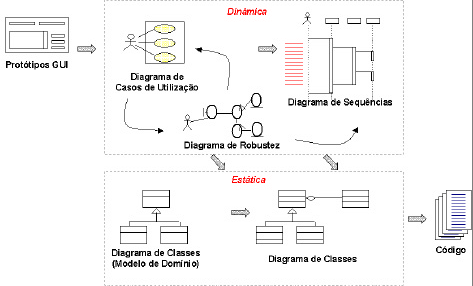
\includegraphics[scale=1.2]{./imagens/iconix1.png}}
  \caption[Visão Geral do ICONIX]
          {Visão Geral do ICONIX. \textbf{Fonte:} \cite{UML_Silva_Videira}}
\label{fig:exemplo1}
\end{figure}

\par A visão gerla do ICONIX pode ser exemplificada na figura 1, identificando a
característica peculiar e a importância de utilizar o UML, levando em
consideração que um sistema gera uma dependência de uma versão mais detalhada
dos diagramas, isso porque é óbivio o uso destes diagramas para implementaçao do
código.

\subsection{Análise de Requisitos}

\par Para realizar a análise de requisitos é necessário que seja realizado
algumas atividades, as quais são descritas a seguir e inlustrado na figura 2.

\begin{figure}[h!]
  \centerline{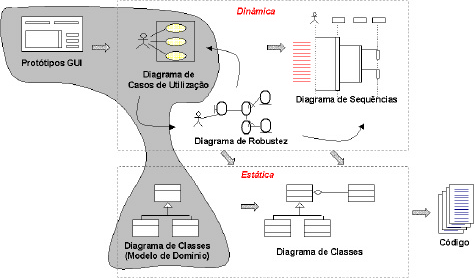
\includegraphics[scale=1.2]{./imagens/iconix2.png}}
  \caption[Tarefa de análise de requisitos]
          {Tarefa de análise de requisitos. \textbf{Fonte:}
          \cite{UML_Silva_Videira}}
\label{fig:exemplo1}
\end{figure}

\begin{itemize}
  \item Fazer com que seja identificados os objetos retirados da realidade,
  assim como todo os atos de relatar compostos na generalização, associação e na
  agregação. Utilizar também o digrama de modelo de domínio que coresponda ao
  diagrama de classe em elevado escalão.
  \item Ao notar orgaçamento suficiênte para desenvolvimento de protótipos que
  utilizam uma interface gráfica ou GUI (\textit{Graphical User   Interface}), 
  a utilização de digramas de navegação, facilitando o intendimento
  do cliente e de seus usuários.
  \item Fazer a identificação dos casos de utilização que estejam diretamente
  ligados ao sistema. Elaborar o digrama de caso de utilização deixando em
  evidência os atores e suas relações que estejam envolvidos.
  \item Fazer um divisão organizada em conjuntos do casos de utilização,
  separando estes conjuntos em digramas de pacotes (\textit{packages}).
  \item Realizar a agremiação de requisitos funcionais com os casos de uso, e
  criando vínculo com os objetos de domínio.
\end{itemize}

\par No processo ICONIX, faz-se distinção clara de um requisito e um caso de
utilização, de acordo com \citeonline[p.378]{UML_Silva_Videira} seguintes
características peculiáres:

\begin{citacao}
     \par Um caso de utilização descreve uma unidade de comportamento.
  	 \par Um requisito descreve uma regra que governa o comportamento.
  	 \par Um caso de utilização satisfaz um ou mais requisitos funcionais.
  	 \par Um requisito funcional pode ser satisfeito por um ou mais casos de
			utilização.
\end{citacao}

\par Assim o processo do ICONIX, tem relações de muitos para muitos no meio de
casos de utilização e os requisitos.

\subsection{Análise e Desenho Preliminar}

\par Para realizar a análise e desenho preliminar é necessário que seja
realizado algumas atividades, as quais são descritas a seguir e inlustrado na
figura 3.

\begin{figure}[h!]
  \centerline{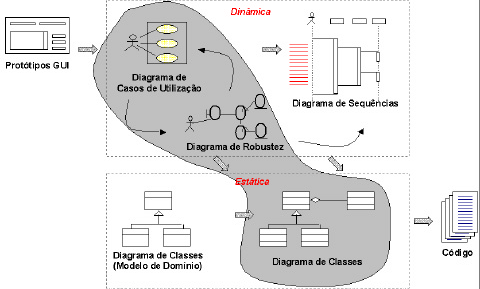
\includegraphics[scale=1.2]{./imagens/iconix3.png}}
  \caption[Tarefa de análise e desenho preliminar]
          {Tarefa de análise e desenho preliminar. \textbf{Fonte:}
          \cite{UML_Silva_Videira}}
\label{fig:exemplo1}
\end{figure}

\begin{itemize}
  			\item Descrever todos os casos de utilização que estivem ligados com os
  			cenários alternativos, cenários de excepção e cenário principal.
  			\item Elabora diagramas de análise de robustez. A cada diagrama de caso de
  			utlização é necessário um diagrama de Robutez 
  			
  			\begin{itemize}
  				\item Fazer a identificação primeiramente do conjunto de objetos,
  				fazendo uso de estereótipos definidos pela UML(), que são as entidades
  				(\textit{entity}), interface/fronteira (\textit{boundary}) e a de controle
  				(\textit{control}), que são espeficados no ``processo de desenvolviemto de
  				software``.
  				\item Fazer a atualização relacionadas ao diagrama de domínio,
  				introduzindo os novos objetos e atributos que foram gerados pelo processo
  				de descoberta.			
			\end{itemize}

  			\item Fazer as atualizações no diagrama de classe de modo que repercuta
  			seus resultados na finalização da fase de análise.
\end{itemize}

\subsection{Desenho}

\par Para realizar o desenho é necessário que seja
realizado algumas atividades, as quais são descritas a seguir e inlustrado na
figura 4.

\begin{figure}[h!]
  \centerline{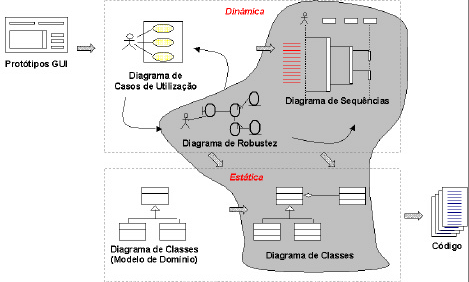
\includegraphics[scale=1.2]{./imagens/iconix4.png}}
  \caption[Tarefa de Desenho]
          {Tarefa de Desenho. \textbf{Fonte:}
          \cite{UML_Silva_Videira}}
\label{fig:exemplo1}
\end{figure}

\begin{itemize}
  \item Cada Caso de tiliação é necessário a a específicação do comportamento.
 	
 	\begin{itemize}
 	  \item  Fazer identificação das mensagens que são enviadas e recebidas entre
 	  métodos e objetos parceiro e que foram invocados, de modo a identificar os
 	  objetos. O diagrama de sequência deve conter ao seu lado direio as
 	  informações textuais do desenho e ao lado esquerdo as informações textuais
 	  do caso de utilização. Continuar a atualização relacionadas ao diagrama de domínio,
  	  introduzindo os novos objetos e atributos que foram gerados pelo processo
  	  de descoberta.
 	  \item Se for necessário pode-se usar digramas de colaboração como forma de
 	  ilustrar as principais transações dos objetos.
 	\end{itemize}
 	
 	\item Finalizar os diagramas que são do modelo estático, e incluir informações
 	detalhadas sobre o diagrama, dentro da visibilidade e dos padrões do desenho.
 	
\end{itemize} 


\subsection{Implementação}

\par Para realizar a implementação é necessário que seja
realizado algumas atividades, as quais são descritas a seguir e inlustrado na
figura 5.

\begin{figure}[h!]
  \centerline{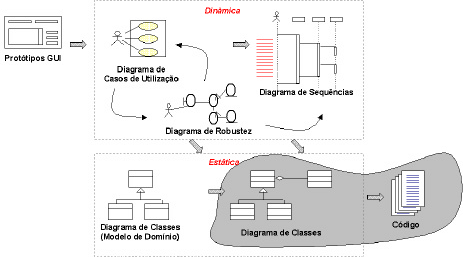
\includegraphics[scale=1.2]{./imagens/iconix5.png}}
  \caption[Tarefa de Implementação]
          {Tarefa de Implementação. \textbf{Fonte:}
          \cite{UML_Silva_Videira}}
\label{fig:exemplo1}
\end{figure}


\begin{itemize}
  \item De acordo com as necessidade do projeto, deve-se elaborar diagramas de
  arquitetura, como por exemplo diagramas de instalação e de componentes, que
  ampare os estágios de implatanção.
  \item Compor códificação e anotações.
  \item Elaborar rotinas de testes, como o cárter unitário e de intergração.
  \item Elaborar rotinas de testes, no sistema como um todo e com foco no
  usuário, visando sua aceitação.
\end{itemize} 


